\documentclass[border=10pt,tikz]{standalone}
\usepackage{tikz}
\usetikzlibrary{shapes,arrows,positioning,calc}

\begin{document}

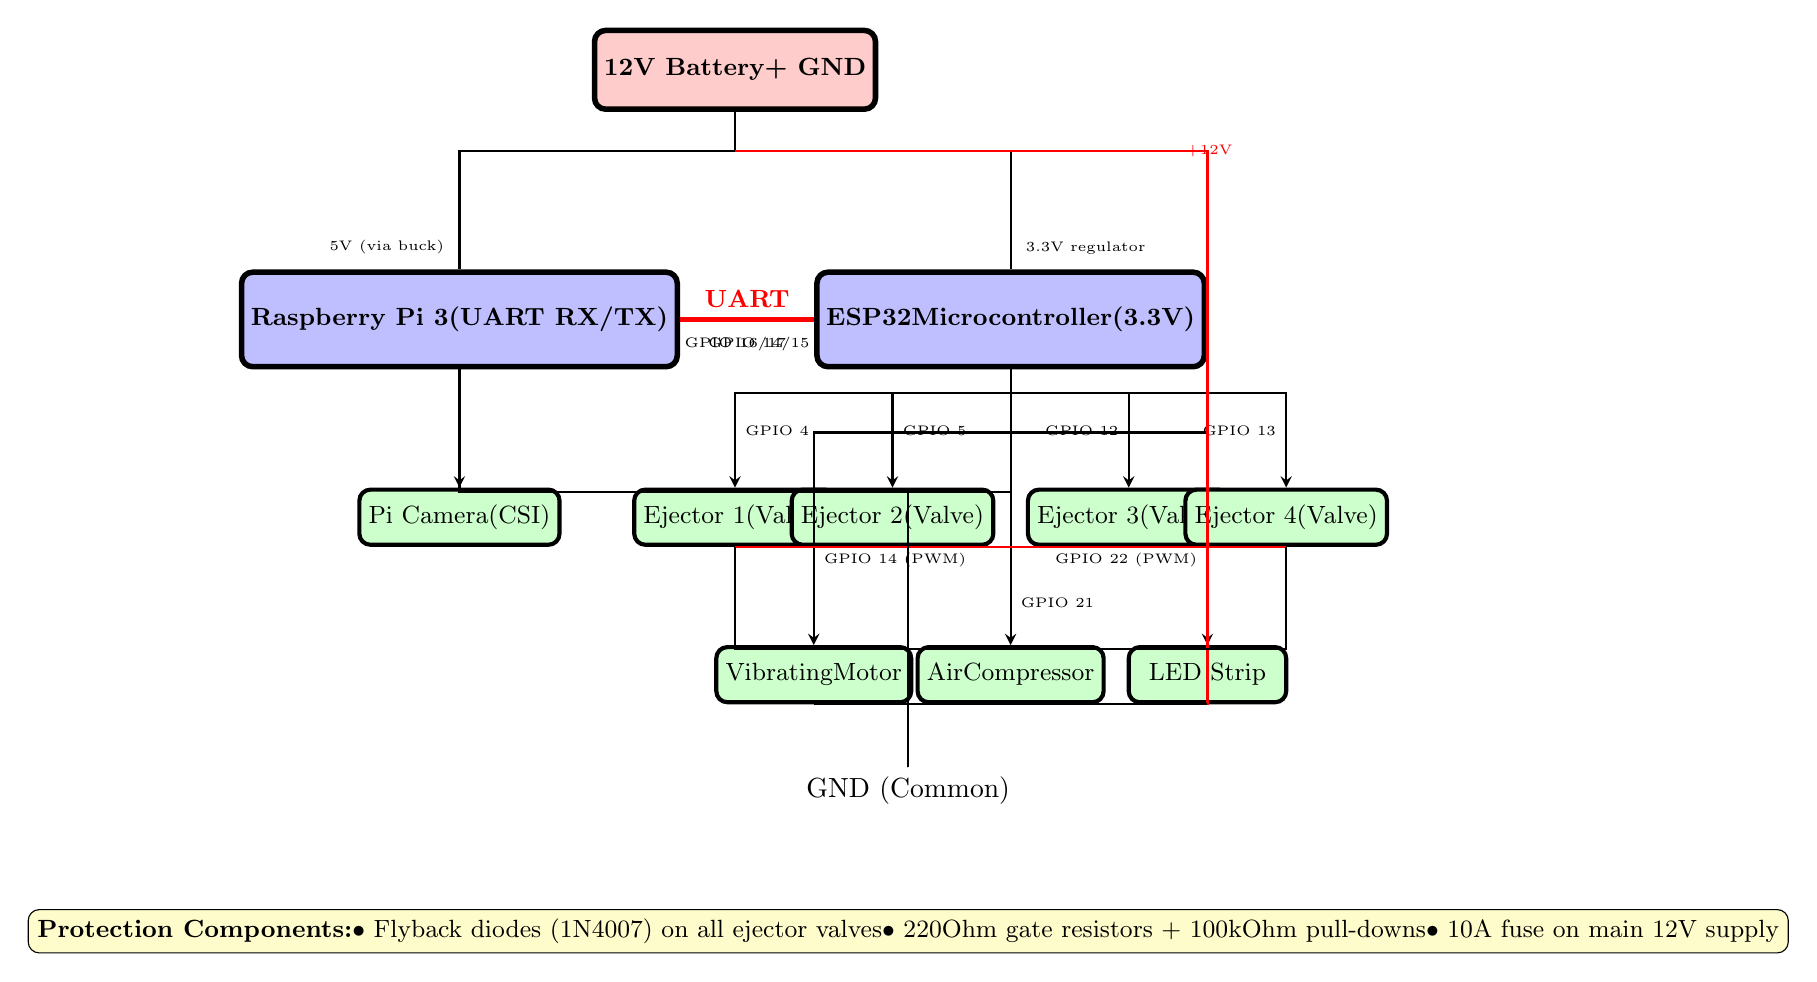
\begin{tikzpicture}[node distance=1.8cm, auto]

% Define styles
\tikzstyle{battery} = [rectangle, rounded corners, minimum width=2.5cm, minimum height=1cm, text centered, draw=black, fill=red!20, line width=2pt, font=\small\bfseries]
\tikzstyle{processor} = [rectangle, rounded corners, minimum width=2.5cm, minimum height=1.2cm, text centered, draw=black, fill=blue!25, line width=2pt, font=\small\bfseries]
\tikzstyle{device} = [rectangle, rounded corners, minimum width=2cm, minimum height=0.7cm, text centered, draw=black, fill=green!20, line width=1.5pt, font=\small]
\tikzstyle{arrow} = [thick, ->, >=stealth]
\tikzstyle{line} = [thick]

% Top: Power Supply
\node (battery) [battery] {12V Battery\\+ GND};

% Processors
\node (pi) [processor, below=2cm of battery, xshift=-3.5cm] {Raspberry Pi 3\\(UART RX/TX)};
\node (esp) [processor, below=2cm of battery, xshift=3.5cm] {ESP32\\Microcontroller\\(3.3V)};

% Power connections
\draw [line] (battery.south) -- ++(0, -0.5) -| (pi.north);
\draw [line] (battery.south) -- ++(0, -0.5) -| (esp.north);
\node [above left=0.1cm of pi.north, font=\tiny] {5V (via buck)};
\node [above right=0.1cm of esp.north, font=\tiny] {3.3V regulator};

% UART Connection
\draw [line, color=red, line width=2pt] (pi.east) -- node[above, font=\small\bfseries, color=red] {UART} (esp.west);
\node [below=0.1cm of pi.east, xshift=1cm, font=\tiny] {GPIO 14/15};
\node [below=0.1cm of esp.west, xshift=-1cm, font=\tiny] {GPIO 16/17};

% ESP32 Outputs - Left side
\node (ejector1) [device, below=1.5cm of esp, xshift=-3.5cm] {Ejector 1\\(Valve)};
\node (ejector2) [device, below=1.5cm of esp, xshift=-1.5cm] {Ejector 2\\(Valve)};
\node (ejector3) [device, below=1.5cm of esp, xshift=1.5cm] {Ejector 3\\(Valve)};
\node (ejector4) [device, below=1.5cm of esp, xshift=3.5cm] {Ejector 4\\(Valve)};

% ESP32 Outputs - Bottom row
\node (motor) [device, below=3.5cm of esp, xshift=-2.5cm] {Vibrating\\Motor};
\node (compressor) [device, below=3.5cm of esp, xshift=0cm] {Air\\Compressor};
\node (led) [device, below=3.5cm of esp, xshift=2.5cm] {LED Strip};

% Pi Camera
\node (camera) [device, below=1.5cm of pi] {Pi Camera\\(CSI)};
\draw [arrow] (pi.south) -- (camera.north);

% Connections from ESP32 to ejectors
\draw [arrow] (esp.south) -- ++(0, -0.3) -| (ejector1.north) node[pos=0.7, right, font=\tiny] {GPIO 4};
\draw [arrow] (esp.south) -- ++(0, -0.3) -| (ejector2.north) node[pos=0.7, right, font=\tiny] {GPIO 5};
\draw [arrow] (esp.south) -- ++(0, -0.3) -| (ejector3.north) node[pos=0.7, left, font=\tiny] {GPIO 12};
\draw [arrow] (esp.south) -- ++(0, -0.3) -| (ejector4.north) node[pos=0.7, left, font=\tiny] {GPIO 13};

% Connections from ESP32 to bottom devices
\draw [arrow] (esp.south) -- ++(0, -0.8) -| (motor.north) node[pos=0.8, right, font=\tiny] {GPIO 14 (PWM)};
\draw [arrow] (esp.south) -- ++(0, -0.8) -- (compressor.north) node[pos=0.8, right, font=\tiny] {GPIO 21};
\draw [arrow] (esp.south) -- ++(0, -0.8) -| (led.north) node[pos=0.8, left, font=\tiny] {GPIO 22 (PWM)};

% Power to devices (12V)
\coordinate (power_junction) at ($(battery.south) + (0, -0.5)$);
\draw [line, color=red] (power_junction) -- ++(6, 0) |- (ejector1.south);
\draw [line, color=red] (power_junction) -- ++(6, 0) |- (ejector2.south);
\draw [line, color=red] (power_junction) -- ++(6, 0) |- (ejector3.south);
\draw [line, color=red] (power_junction) -- ++(6, 0) |- (ejector4.south);
\draw [line, color=red] (power_junction) -- ++(6, 0) |- (motor.south);
\draw [line, color=red] (power_junction) -- ++(6, 0) |- (compressor.south);
\draw [line, color=red] (power_junction) -- ++(6, 0) |- (led.south);
\node [right=0.1cm of power_junction, xshift=5.5cm, font=\tiny, color=red] {+12V};

% Ground connections
\node (gnd) [below=0.8cm of motor, xshift=1.2cm] {GND (Common)};
\draw [line] (gnd.north) |- (motor.south);
\draw [line] (gnd.north) |- (compressor.south);
\draw [line] (gnd.north) |- (led.south);
\draw [line] (gnd.north) |- ++(0, 1.5) -| (ejector1.south);
\draw [line] (gnd.north) |- ++(0, 1.5) -| (ejector4.south);
\draw [line] (gnd.north) |- ++(0, 3.5) -| (pi.south);
\draw [line] (gnd.north) |- ++(0, 3.5) -| (esp.south);

% Protection note
\node [draw=black, fill=yellow!20, rounded corners, below=1.2cm of gnd, minimum width=7cm, font=\small] {
\textbf{Protection Components:} \\
$\bullet$ Flyback diodes (1N4007) on all ejector valves \\
$\bullet$ 220Ohm gate resistors + 100kOhm pull-downs \\
$\bullet$ 10A fuse on main 12V supply
};

\end{tikzpicture}

\end{document}
